\chapter*{DIAGRAMA DE CASOS DE USO}

\rowcolors{2}{gray!10}{gray!40}



\begin{figure}[ht]
	\centering
	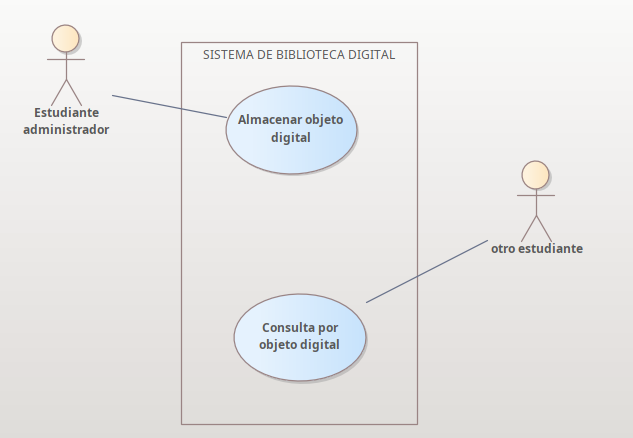
\includegraphics[scale=0.8]{images/casoUso2}
	\caption{Diagrama de casos de uso}
\end{figure}
\begin{center}
\begin{tabular}{lp{10cm}}
    Id del caso de uso & CU-1 \\
    \hline
    Caso de uso & Almacenar objeto digital \\
    Actores & Estudiante administrador \\
    Descripción & Almacena cualquier documento o objeto digital como libros, artículos, videos, audio para poder almacenar un objeto digital (documento o multimedia)  \\
    Precondición & Usuario ingresa al sistema de forma remota, local o por navegador \\
    Post condición & Almacenamiento actualizado \\
\end{tabular}\\
\vspace{0.5cm}
\begin{tabular}{lp{10cm}}
    Id del caso de uso & CU-2 \\
    \hline
    Caso de uso & Consultar por un objeto digital \\
    Actores & Otro estudiante \\
    Descripción & Consulta por cualquier documento o objeto digital como libros, artículos, videos, audio  \\
    Precondición & El estudiante bebe ingresar al sistema\\
    Post condición & Necesidad de información satisfecha \\
\end{tabular}
\end{center}
